\section{Synthetic model and outcome identification}
\label{app:synthetic}
\subsection{The synthetic experiment}
Write $s_y=2y-1$ and $a(v)=\operatorname{expit}((v-1.5)/0.3)$. The simulations use
\begin{align}
 Z\mid k=1,y,v,\theta&\sim N\!\left(s_y\mu(1-e^{-0.1v}),\frac{0.3^2}{1+0.05v}\right),\nonumber\\
 Z\mid k=2,y,v,\theta&\sim N(0,0.5^2),\label{eq:example}\\
 Z\mid k=3,y,v,\theta&\sim -s_y\,0.3a(v)+0.4\,t_5,\nonumber
\end{align}
where $0.4$ is the scale of the Student distribution. The gate has exponents $(0.5,0,0.3)$:
\[
 \rho_k(v;\theta)=\frac{\omega_k(1+v)^{\gamma_k}}{\sum_j\omega_j(1+v)^{\gamma_j}},\qquad
 (\omega_1,\omega_2,\omega_3)=\left(w,\tfrac{2(1-w)}3,\tfrac{1-w}3\right).
\]
The nuisance parameter is $\theta=(w,\mu)$. Volumes are i.i.d.\ Gamma$(2,0.5)$ and $p_0=\pi_0=1/2$. Each scenario uses 2,000 test histories, balanced across outcomes, at horizons $T\in\{10,25,50,100,200,500\}$. The fixed-default scenario sets $(w,\mu)=(0.4,0.5)$. The prior-predictive scenario draws one state per history from the uniform prior on $\{0.15,0.4,0.65\}\times\{0.25,0.5,0.75\}$. Marginal likelihoods sum the nine full-path likelihoods in log space, which is exact integration for a discrete prior. The calibrated endpoint is an intercept and slope on the terminal logit, fitted on a separate set of 2,000 training histories per scenario and horizon. The two ablations replace volume by $1$ or the Student component by a variance-matched Gaussian.

\subsection{Outcome identification}
Let $P_{y,\theta}^{(T)}$ be the product law of Assumption~\ref{ass:product}. At truth $(y^*,\theta^*)$ define
\begin{equation}
 \delta_T=\inf_{\theta\in\Theta}\frac1T\KL\!\left(P_{y^*,\theta^*}^{(T)}\,\middle\|\,P_{1-y^*,\theta}^{(T)}\right).
 \label{eq:gap}
\end{equation}
The same nuisance value must explain the whole path. Outcome identification differs from endpoint sufficiency: a full history may separate outcomes while its endpoint discards information.

\begin{proposition}[Orientation symmetry]
\label{prop:symmetry}
Suppose $\Psi:\Theta\to\Theta$ is a measurable involution and $f_1(\cdot\mid v,\theta)=f_0(\cdot\mid v,\Psi\theta)$ on the design. Then $\delta_T=0$ at every truth. If also $\Pi\circ\Psi^{-1}=\Pi$, then $m_{1,T}=m_{0,T}$ for every path and $\pi_T=\pi_0$ for every $T$.
\end{proposition}
\begin{proof}
The opposite outcome with parameter $\Psi\theta^*$ reproduces the true law. Changing variables by $\Psi$ in the marginal likelihood and using prior invariance proves the second assertion.
\end{proof}
An unknown common orientation multiplying both directional means in \eqref{eq:example}, with equal prior mass on $+1$ and $-1$, gives this symmetry. Restricting the orientation removes it and is a substantive prior restriction.

\begin{proposition}[A checkable separation condition]
\label{prop:sign}
Let $I_T\subset\{1,\ldots,T\}$. Suppose that for each $t\in I_T$ there is a measurable set $A_t$ and a constant $d>0$, uniform in $T$, such that
\[
 P_{y^*,\theta^*}(Z_t\in A_t)\geq b_t+d,\qquad
 \sup_{\theta\in\Theta}P_{1-y^*,\theta}(Z_t\in A_t)\leq b_t.
\]
Then $\delta_T\geq 2d^2|I_T|/T$.
\end{proposition}
\begin{proof}
The difference on $A_t$ bounds total variation below by $d$. Pinsker's inequality bounds each relevant KL divergence below by $2d^2$. Sum these bounds before taking the infimum in \eqref{eq:gap}.
\end{proof}

\subsection{Horizon scores and oracle endpoint posteriors}
\begin{figure}[h]
\centering
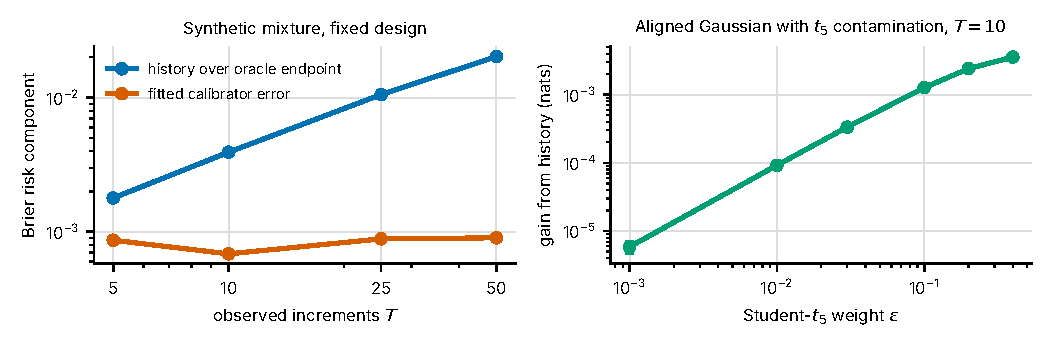
\includegraphics[width=\linewidth]{generated/oracle_endpoint.pdf}
\caption{Left: Brier components of Proposition~\ref{prop:decomposition} for the synthetic mixture at fixed design, comparing the exact history posterior with the numerically approximated oracle endpoint posterior (blue) and the error of a fitted intercept-and-slope endpoint calibrator (orange). Right: gain from history in an aligned Gaussian model with a centered Student-$t_5$ contamination of weight $\varepsilon$, with $\pm2$ Monte Carlo standard errors. The left panel uses $40{,}000$ histories per point. The right panel uses stratified sampling on the number of contaminated increments for $\varepsilon\le0.1$ and $400{,}000$ plain draws above.}
\label{fig:oracle}
\end{figure}
\begin{figure}[t]
\centering
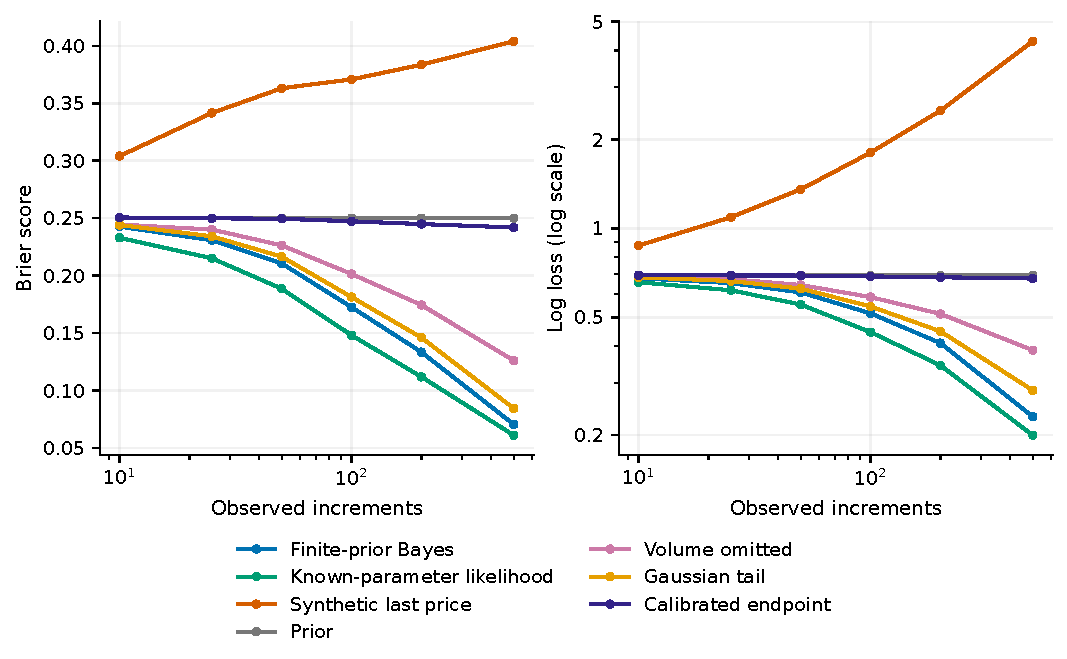
\includegraphics[width=\linewidth]{generated/revised_scores.pdf}
\caption{Synthetic proper scores against horizon under prior-predictive simulation. The calibrated endpoint uses independent training histories. Lines show sample means over 2,000 histories. The right panel has a logarithmic vertical axis.}
\label{fig:scores}
\end{figure}
For the oracle comparison of Sect.~\ref{sec:synthetic} the design is fixed at $v_t\equiv1$. For each outcome and nuisance state, the one-step density is evaluated on a grid of spacing $h=0.002$ over $[-L_T,L_T]$ with $L_T=0.15T+5\sqrt T+25$, normalized, and raised to the $T$-th power in the Fourier domain. The endpoint density is the uniform mixture of the nine convolved densities, and $r^*$ is obtained by linear interpolation of the two log densities at the observed sum. Repeating the computation with $h=0.001$ on $[-1.5L_T,1.5L_T]$ changes $r^*$ by at most $3.7\times10^{-8}$ on the simulated histories and the reported gains by less than $10^{-11}$. Monte Carlo standard errors of the intrinsic gains are at most $1.2\times10^{-4}$ (Brier) and $2.8\times10^{-4}$ nats (log). The endpoint calibrator is an unpenalized intercept-and-slope logistic regression on $S$, fitted on $2{,}000$ independent histories.

The contamination study uses the same convolution with a single state, $Z_t\mid Y\sim(1-\varepsilon)N(s_Y0.1,0.5^2)+\varepsilon\,0.5\sqrt{3/5}\,t_5$ and $T=10$, on $[-1.5L,1.5L]$ with $L=20+3\sqrt{10}$ and $h=0.001$, which agrees with the coarser grid to within $5\times10^{-8}$ in $r^*$. Plain Monte Carlo is unreliable at small $\varepsilon$ because the gain comes from rare large draws. For $\varepsilon\le0.1$ we therefore stratify on the number $K$ of contaminated increments, draw $10^5$ histories with $K=k$ for $k=0,\ldots,5$, and weight the stratum means by the Binomial$(10,\varepsilon)$ probabilities. The omitted mass $\Prob(K>5)$ is at most $1.5\times10^{-4}$. The resulting gains are $9.2\times10^{-5}$ ($\pm0.7\times10^{-5}$), $3.34\times10^{-4}$ ($\pm0.16\times10^{-4}$) and $1.27\times10^{-3}$ ($\pm0.03\times10^{-3}$) at $\varepsilon=0.01$, $0.03$ and $0.1$. At $\varepsilon=0.001$ three independent runs, with $10^5$ or $10^6$ draws per stratum, gave $5.9$, $6.3$ and $7.1\times10^{-6}$, a spread larger than their nominal standard errors, so we report only the order of magnitude. Above $\varepsilon=0.1$ we use $400{,}000$ plain draws.
